\documentclass{standalone}
\usepackage{tikz}
\usetikzlibrary{patterns, positioning}


\begin{document}
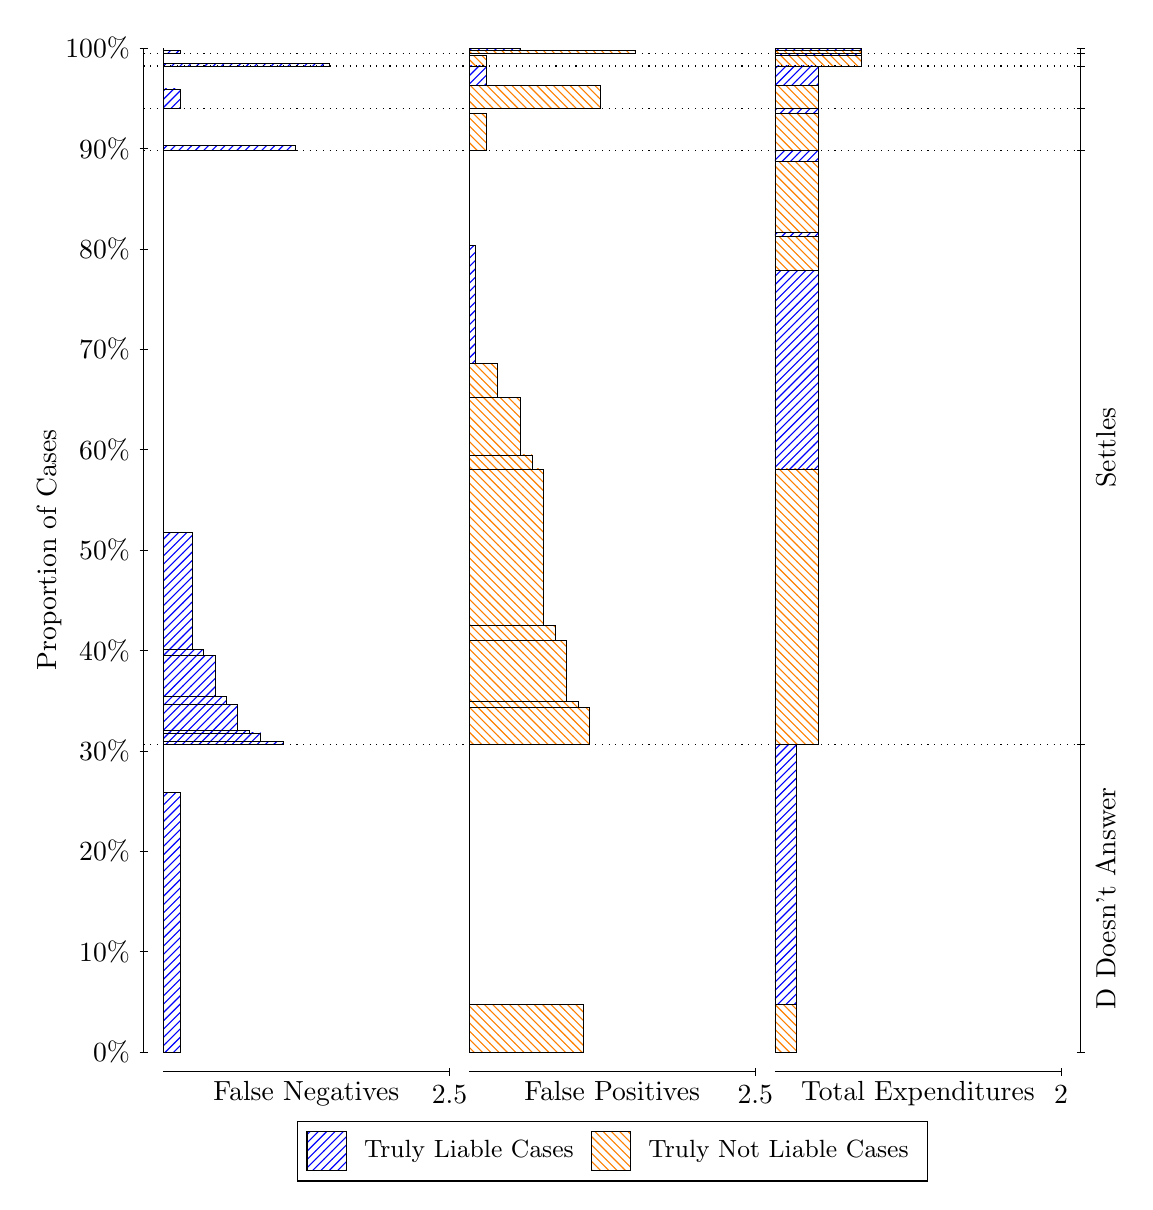
\begin{tikzpicture}
\draw[black, very thin] (1.5,1.75) -- (1.5,14.5);
\node[rotate=90, text=black, anchor=center] at (0.3, 8.125) {Proportion of Cases};
\draw[black, very thin] (1.45,1.75) -- (1.55,1.75);
\node[text=black, anchor=east] at (1.45, 1.75) {0\%};
\draw[black, very thin] (1.45,3.025) -- (1.55,3.025);
\node[text=black, anchor=east] at (1.45, 3.025) {10\%};
\draw[black, very thin] (1.45,4.3) -- (1.55,4.3);
\node[text=black, anchor=east] at (1.45, 4.3) {20\%};
\draw[black, very thin] (1.45,5.575) -- (1.55,5.575);
\node[text=black, anchor=east] at (1.45, 5.575) {30\%};
\draw[black, very thin] (1.45,6.85) -- (1.55,6.85);
\node[text=black, anchor=east] at (1.45, 6.85) {40\%};
\draw[black, very thin] (1.45,8.125) -- (1.55,8.125);
\node[text=black, anchor=east] at (1.45, 8.125) {50\%};
\draw[black, very thin] (1.45,9.4) -- (1.55,9.4);
\node[text=black, anchor=east] at (1.45, 9.4) {60\%};
\draw[black, very thin] (1.45,10.675) -- (1.55,10.675);
\node[text=black, anchor=east] at (1.45, 10.675) {70\%};
\draw[black, very thin] (1.45,11.95) -- (1.55,11.95);
\node[text=black, anchor=east] at (1.45, 11.95) {80\%};
\draw[black, very thin] (1.45,13.225) -- (1.55,13.225);
\node[text=black, anchor=east] at (1.45, 13.225) {90\%};
\draw[black, very thin] (1.45,14.5) -- (1.55,14.5);
\node[text=black, anchor=east] at (1.45, 14.5) {100\%};

\draw[black, very thin] (13.4,1.75) -- (13.4,14.5);
\draw[black, very thin] (13.35,1.75) -- (13.45,1.75);
\node[anchor=west] at (13.35, 1.75) {};
\draw[black, very thin] (13.35,5.6538) -- (13.45,5.6538);
\node[anchor=west] at (13.35, 5.6538) {};
\draw[black, very thin] (13.35,13.198) -- (13.45,13.198);
\node[anchor=west] at (13.35, 13.198) {};
\draw[black, very thin] (13.35,13.732) -- (13.45,13.732);
\node[anchor=west] at (13.35, 13.732) {};
\draw[black, very thin] (13.35,14.272) -- (13.45,14.272);
\node[anchor=west] at (13.35, 14.272) {};
\draw[black, very thin] (13.35,14.435) -- (13.45,14.435);
\node[anchor=west] at (13.35, 14.435) {};
\draw[black, very thin] (13.35,14.5) -- (13.45,14.5);
\node[anchor=west] at (13.35, 14.5) {};

\draw[black, very thin, pattern color=blue, pattern=north east lines] (1.75,1.75) rectangle (1.968,5.0508);
\draw[black, very thin, pattern color=orange, pattern=north west lines] (1.75,5.0508) rectangle (1.75,5.6538);
\draw[black, very thin, pattern color=blue, pattern=north east lines] (1.75,5.6538) rectangle (3.276,5.6975);
\draw[black, very thin, pattern color=blue, pattern=north east lines] (1.75,5.6975) rectangle (2.9853,5.8031);
\draw[black, very thin, pattern color=blue, pattern=north east lines] (1.75,5.8031) rectangle (2.84,5.8307);
\draw[black, very thin, pattern color=blue, pattern=north east lines] (1.75,5.8307) rectangle (2.6947,6.1684);
\draw[black, very thin, pattern color=blue, pattern=north east lines] (1.75,6.1684) rectangle (2.5493,6.2704);
\draw[black, very thin, pattern color=blue, pattern=north east lines] (1.75,6.2704) rectangle (2.404,6.7882);
\draw[black, very thin, pattern color=blue, pattern=north east lines] (1.75,6.7882) rectangle (2.2587,6.8622);
\draw[black, very thin, pattern color=blue, pattern=north east lines] (1.75,6.8622) rectangle (2.1133,8.3536);
\draw[black, very thin, pattern color=orange, pattern=north west lines] (1.75,8.3536) rectangle (1.75,13.198);
\draw[black, very thin, pattern color=blue, pattern=north east lines] (1.75,13.198) rectangle (3.4213,13.259);
\draw[black, very thin, pattern color=orange, pattern=north west lines] (1.75,13.259) rectangle (1.75,13.732);
\draw[black, very thin, pattern color=blue, pattern=north east lines] (1.75,13.732) rectangle (1.968,13.98);
\draw[black, very thin, pattern color=orange, pattern=north west lines] (1.75,13.98) rectangle (1.75,14.272);
\draw[black, very thin, pattern color=blue, pattern=north east lines] (1.75,14.272) rectangle (3.8573,14.305);
\draw[black, very thin, pattern color=orange, pattern=north west lines] (1.75,14.305) rectangle (1.75,14.435);
\draw[black, very thin, pattern color=blue, pattern=north east lines] (1.75,14.435) rectangle (1.968,14.467);
\draw[black, very thin, pattern color=orange, pattern=north west lines] (1.75,14.467) rectangle (1.75,14.5);
\draw[black, very thin, pattern color=orange, pattern=north west lines] (5.6333,1.75) rectangle (7.0867,2.353);
\draw[black, very thin, pattern color=blue, pattern=north east lines] (5.6333,2.353) rectangle (5.6333,5.6538);
\draw[black, very thin, pattern color=orange, pattern=north west lines] (5.6333,5.6538) rectangle (7.1593,6.1251);
\draw[black, very thin, pattern color=orange, pattern=north west lines] (5.6333,6.1251) rectangle (7.014,6.2051);
\draw[black, very thin, pattern color=orange, pattern=north west lines] (5.6333,6.2051) rectangle (6.8687,6.977);
\draw[black, very thin, pattern color=orange, pattern=north west lines] (5.6333,6.977) rectangle (6.7233,7.1671);
\draw[black, very thin, pattern color=orange, pattern=north west lines] (5.6333,7.1671) rectangle (6.578,9.1539);
\draw[black, very thin, pattern color=orange, pattern=north west lines] (5.6333,9.1539) rectangle (6.4327,9.3325);
\draw[black, very thin, pattern color=orange, pattern=north west lines] (5.6333,9.3325) rectangle (6.2873,10.065);
\draw[black, very thin, pattern color=orange, pattern=north west lines] (5.6333,10.065) rectangle (5.9967,10.499);
\draw[black, very thin, pattern color=blue, pattern=north east lines] (5.6333,10.499) rectangle (5.706,11.99);
\draw[black, very thin, pattern color=blue, pattern=north east lines] (5.6333,11.99) rectangle (5.6333,13.198);
\draw[black, very thin, pattern color=orange, pattern=north west lines] (5.6333,13.198) rectangle (5.8513,13.671);
\draw[black, very thin, pattern color=blue, pattern=north east lines] (5.6333,13.671) rectangle (5.6333,13.732);
\draw[black, very thin, pattern color=orange, pattern=north west lines] (5.6333,13.732) rectangle (7.3047,14.024);
\draw[black, very thin, pattern color=blue, pattern=north east lines] (5.6333,14.024) rectangle (5.8513,14.272);
\draw[black, very thin, pattern color=orange, pattern=north west lines] (5.6333,14.272) rectangle (5.8513,14.402);
\draw[black, very thin, pattern color=blue, pattern=north east lines] (5.6333,14.402) rectangle (5.6333,14.435);
\draw[black, very thin, pattern color=orange, pattern=north west lines] (5.6333,14.435) rectangle (7.7407,14.467);
\draw[black, very thin, pattern color=blue, pattern=north east lines] (5.6333,14.467) rectangle (6.2873,14.5);
\draw[black, very thin, pattern color=orange, pattern=north west lines] (9.5167,1.75) rectangle (9.7892,2.353);
\draw[black, very thin, pattern color=blue, pattern=north east lines] (9.5167,2.353) rectangle (9.7892,5.6538);
\draw[black, very thin, pattern color=orange, pattern=north west lines] (9.5167,5.6538) rectangle (10.062,9.1539);
\draw[black, very thin, pattern color=blue, pattern=north east lines] (9.5167,9.1539) rectangle (10.062,11.677);
\draw[black, very thin, pattern color=orange, pattern=north west lines] (9.5167,11.677) rectangle (10.062,12.111);
\draw[black, very thin, pattern color=blue, pattern=north east lines] (9.5167,12.111) rectangle (10.062,12.154);
\draw[black, very thin, pattern color=orange, pattern=north west lines] (9.5167,12.154) rectangle (10.062,13.065);
\draw[black, very thin, pattern color=blue, pattern=north east lines] (9.5167,13.065) rectangle (10.062,13.198);
\draw[black, very thin, pattern color=orange, pattern=north west lines] (9.5167,13.198) rectangle (10.062,13.671);
\draw[black, very thin, pattern color=blue, pattern=north east lines] (9.5167,13.671) rectangle (10.062,13.732);
\draw[black, very thin, pattern color=orange, pattern=north west lines] (9.5167,13.732) rectangle (10.062,14.024);
\draw[black, very thin, pattern color=blue, pattern=north east lines] (9.5167,14.024) rectangle (10.062,14.272);
\draw[black, very thin, pattern color=orange, pattern=north west lines] (9.5167,14.272) rectangle (10.607,14.402);
\draw[black, very thin, pattern color=blue, pattern=north east lines] (9.5167,14.402) rectangle (10.607,14.435);
\draw[black, very thin, pattern color=orange, pattern=north west lines] (9.5167,14.435) rectangle (10.607,14.467);
\draw[black, very thin, pattern color=blue, pattern=north east lines] (9.5167,14.467) rectangle (10.607,14.5);
\draw[black, dotted] (1.5,5.6538) -- (13.4,5.6538);
\draw[black, dotted] (1.5,13.198) -- (13.4,13.198);
\draw[black, dotted] (1.5,13.732) -- (13.4,13.732);
\draw[black, dotted] (1.5,14.272) -- (13.4,14.272);
\draw[black, dotted] (1.5,14.435) -- (13.4,14.435);
\draw[black, very thin] (1.75,1.5) -- (5.3833,1.5);
\node[text=black, anchor=north] at (3.5667, 1.5) {False Negatives};
\draw[black, very thin] (5.3833,1.45) -- (5.3833,1.55);
\node[text=black, anchor=north] at (5.3833, 1.45) {2.5};

\draw[black, very thin] (5.6333,1.5) -- (9.2667,1.5);
\node[text=black, anchor=north] at (7.45, 1.5) {False Positives};
\draw[black, very thin] (9.2667,1.45) -- (9.2667,1.55);
\node[text=black, anchor=north] at (9.2667, 1.45) {2.5};

\draw[black, very thin] (9.5167,1.5) -- (13.15,1.5);
\node[text=black, anchor=north] at (11.333, 1.5) {Total Expenditures};
\draw[black, very thin] (13.15,1.45) -- (13.15,1.55);
\node[text=black, anchor=north] at (13.15, 1.45) {2};

\node[text=black, centered, rotate=90] at (13.72, 3.7019) {D Doesn't Answer};
\node[text=black, centered, rotate=90] at (13.72, 9.426) {Settles};





\draw (7.449999999999999,1.5) node[draw=none] (baseCoordinate) {};
\begin{scope}[align=center]
        \matrix[scale=0.5, draw=black, below=0.5cm of baseCoordinate, nodes={draw}, column sep=0.1cm]{
            \node[rectangle, draw, minimum width=0.5cm, minimum height=0.5cm, pattern color=blue, pattern=north east lines] {}; &
            \node[draw=none, font=\small, text=black] (B) {Truly Liable Cases}; &
            \node[rectangle, draw, minimum width=0.5cm, minimum height=0.5cm, pattern color=orange, pattern=north west lines] {}; &
            \node[draw=none, font=\small, text=black] (B) {Truly Not Liable Cases}; \\
            };
\end{scope}

\end{tikzpicture}
\end{document}